Sparse coding has been observed in neurons in the visual tract \citep{OlshausenField2004a}, a simple model is proposed for such neurons.

It is unlikely that a neuron is ever truly ``off'', so it is assumed that a neuron has a base-firing state that will be referred to as the ``off-state''.  For the sake of simplicity, it is assumed that a neuron in such an ``off-state'' would have a constant firing rate, $\lambda_d$.  Correspondingly, for sparse-coding a neuron must have a higher firing-rate when the feature that it codes for is present; this firing rate, $\lambda_u$, is also taken to be constant.


This idea is simplified to the extreme case, where a neuron is either in its up-state and has a high firing-rate, or it is ``off''.   The model is treated as a Poisson process, for ease of calculation.


The data that is simulated has an ``up rate'' $\lambda_u$ and a ``down rate'' $\lambda_d$.  For the initial trials, $\lambda_d = 0$.  When in the down-state, the state switches ``up'' with expected frequency $u$, and when in the up-state it switches ``down'' with expected frequency $d$.  Thus, the average background rate, $r$, of the inhomogeneous Poisson process can be calculated as:
\begin{equation}\label{lam}
r = \frac{ \frac{\lambda_u }{d}}{ \frac{1}{u} + \frac{1}{d}} = \frac{u\, \lambda_u}{u+d}
\end{equation}
since the expected time for being in the up-state is simply $1/d$ and the expected time in the down-state is $1/u$.

\begin{figure}[htb]
\begin{center}
\setlength{\unitlength}{.08cm}
\begin{picture}(150,75)
\put(0,14){\mbox{$\lambda_d$}}
\put(0,34){\mbox{$\lambda_u$}}

\linethickness{1.5pt}
\put(7,10){\line(1,0){138}}
\put(7,55){\line(1,0){138}}

\linethickness{1pt}
\put(7,15){\line(1,0){18}}
\put(15,15){\vector(0,1){8}}
\put(17,17){\mbox{$u$}}
\put(25,15){\line(0,1){20}}
\put(25,35){\line(1,0){30}}
\put(38,35){\vector(0,-1){8}}
\put(40,30){\mbox{$d$}}
\put(55,35){\line(0,-1){20}}
\put(55,15){\line(1,0){40}}
\put(73,15){\vector(0,1){8}}
\put(75,17){\mbox{$u$}}
\put(95,15){\line(0,1){20}}
\put(95,35){\line(1,0){25}}
\put(106,35){\vector(0,-1){8}}
\put(108,30){\mbox{$d$}}
\put(120,35){\line(0,-1){20}}
\put(120,15){\line(1,0){25}}
\put(132,15){\vector(0,1){8}}
\put(134,17){\mbox{$u$}}

\put(27,55){\line(0,1){15}}
\put(35,55){\line(0,1){15}}
\put(46,55){\line(0,1){15}}
\put(50,55){\line(0,1){15}}

\put(67,55){\line(0,1){15}}
\put(84,55){\line(0,1){15}}

\put(100,55){\line(0,1){15}}
\put(107,55){\line(0,1){15}}
\put(116,55){\line(0,1){15}}
\put(135,55){\line(0,1){15}}

\multiput(8,35)(5,0){28}{\line(1,0){2}}
%\multiput(8,15)(5,0){28}{\line(1,0){2}}
\end{picture}
\bigskip
\rule{33em}{0.5pt}
\caption{ \label{model}An illustration of the model firing rate, and an associated output spike train.  The process has two states, an up-state and a down-state, and has Poisson transition rates: $u$ from down to up, and $d$ from up to down.  Each state has an associated Poisson firing rate: $\lambda_u$ when up and $\lambda_d$ when down.  }
\end{center}
\end{figure}


\section{Estimating the firing rate $r(t)$}

With the model for the firing rate as above, it is possible to explicitly calculate the probability of being in the up-state for the time following a spike.  In the initial setting, where $\lambda_d$ is set to zero, then it is known that when there is a spike that the rate is in the up-state, so at the time of spiking $t_0$ the probability $p(t_0)$ of being in the up-state is equal to one.  

For the estimate of the rate, $\tilde{r}(t)$, this is reflected by setting $\tilde{r}(t_0) = \lambda_u$.  The probability is reset  to one every time there is a spike, so it is only required to calculate the probability of being in the up-state given that there has been no spike since the time, $t_0$, of the last spike.  

It is possible, using Bayes' Theorem, to calculate a first approximation of the probability of being in the up-state at a time $t+\Delta t$, given a spike at time $t=t_0$ for small $\Delta t$.

 Let $X=$ up at $t=t_0+\Delta t$, $Y=$ no spike since $t=t_0$ and $Z=$ spike at $t=t_0$. Then,
\begin{equation}\label{p}
P(X|Y|Z) = \frac{P(Y|X,Z)P(X|Z)}{P(Y|Z)} = \frac{(1-\lambda_u \Delta t) (1-d \Delta t)}{1-r\Delta t}
\end{equation}

Then, it is possible to calculate the first approximation to the probability  of being up at time $t$, by letting $t_0=0, \,\Delta t =t/n$.

\begin{equation}
P(\mbox{up at } t | Y , Z)   =  \lim_{n \rightarrow \infty}\prod_{k=1}^n \frac{(1-\lambda_ut/n)(1-dt/n)}{1-rt/n}
\end{equation} 
in the limit as $n$ goes to infinity all terms smaller than $1/n$ are disregarded, so:
\begin{equation}
\begin{split}
P(\mbox{up at } t | Y , Z) &= \lim_{n \rightarrow \infty} \prod_{k=1}^n \left(1+ t\frac{r-\lambda_u-d}{n}\right) \\
& = \lim_{n \rightarrow \infty} \left(1 + t\frac{r-\lambda_u -d}{n} \right)^n \\
\end{split}
\end{equation}
This is the famous limit form of calculating the exponential function, so:
\begin{equation}
P(\mbox{up at } t | Y,Z) = \exp [ (r-\lambda_u-d) ]
\end{equation} 

Recalling from equation \ref{lam} that $\lambda_u = r(u+d)/u$, get:
\begin{equation}
p=e^{-\frac{d(r+u)}{u}(t-t_0)}
\end{equation}

Comparing this to the exponential kernel in the Van Rossum metric \citep{VanRossum2001a}, then:
\begin{equation}
\tau = \frac{u}{d(r+u)}
\end{equation}

This is clearly just the first approximation, since it does not take into account the possibility of the model switching into the down-state and back up.  To calculate the full probability, let $y(t) = P(\mbox{up at } t | Y , Z)$, with $Y,Z$ as in equation \ref{p} above.  Then:

\begin{equation}
\begin{split}
y(t+h) &=  y(t)P(\mbox{staying in up-state} | \mbox{up at t}|Y,Z)  \\
& + (1-y(t))P(\mbox{switching up} | \mbox{down at t}|Y,Z)\\
&\\
&= y(t)\left( \frac{(1-dh)(1-\lambda_uh)}{1-rh} \right) + (1-y(t)) \left(\frac{(uh)(1)}{1-rh}  \right)\\
&\\
& = y(t)\left( 1 + h(r-d-\lambda_u-u ) \right) + uh
\end{split}
\end{equation}

\begin{figure}[b!]
\begin{center}
\resizebox{0.75\textwidth}{!}{% GNUPLOT: LaTeX picture with Postscript
\begingroup
  \makeatletter
  \providecommand\color[2][]{%
    \GenericError{(gnuplot) \space\space\space\@spaces}{%
      Package color not loaded in conjunction with
      terminal option `colourtext'%
    }{See the gnuplot documentation for explanation.%
    }{Either use 'blacktext' in gnuplot or load the package
      color.sty in LaTeX.}%
    \renewcommand\color[2][]{}%
  }%
  \providecommand\includegraphics[2][]{%
    \GenericError{(gnuplot) \space\space\space\@spaces}{%
      Package graphicx or graphics not loaded%
    }{See the gnuplot documentation for explanation.%
    }{The gnuplot epslatex terminal needs graphicx.sty or graphics.sty.}%
    \renewcommand\includegraphics[2][]{}%
  }%
  \providecommand\rotatebox[2]{#2}%
  \@ifundefined{ifGPcolor}{%
    \newif\ifGPcolor
    \GPcolorfalse
  }{}%
  \@ifundefined{ifGPblacktext}{%
    \newif\ifGPblacktext
    \GPblacktexttrue
  }{}%
  % define a \g@addto@macro without @ in the name:
  \let\gplgaddtomacro\g@addto@macro
  % define empty templates for all commands taking text:
  \gdef\gplbacktext{}%
  \gdef\gplfronttext{}%
  \makeatother
  \ifGPblacktext
    % no textcolor at all
    \def\colorrgb#1{}%
    \def\colorgray#1{}%
  \else
    % gray or color?
    \ifGPcolor
      \def\colorrgb#1{\color[rgb]{#1}}%
      \def\colorgray#1{\color[gray]{#1}}%
      \expandafter\def\csname LTw\endcsname{\color{white}}%
      \expandafter\def\csname LTb\endcsname{\color{black}}%
      \expandafter\def\csname LTa\endcsname{\color{black}}%
      \expandafter\def\csname LT0\endcsname{\color[rgb]{1,0,0}}%
      \expandafter\def\csname LT1\endcsname{\color[rgb]{0,1,0}}%
      \expandafter\def\csname LT2\endcsname{\color[rgb]{0,0,1}}%
      \expandafter\def\csname LT3\endcsname{\color[rgb]{1,0,1}}%
      \expandafter\def\csname LT4\endcsname{\color[rgb]{0,1,1}}%
      \expandafter\def\csname LT5\endcsname{\color[rgb]{1,1,0}}%
      \expandafter\def\csname LT6\endcsname{\color[rgb]{0,0,0}}%
      \expandafter\def\csname LT7\endcsname{\color[rgb]{1,0.3,0}}%
      \expandafter\def\csname LT8\endcsname{\color[rgb]{0.5,0.5,0.5}}%
    \else
      % gray
      \def\colorrgb#1{\color{black}}%
      \def\colorgray#1{\color[gray]{#1}}%
      \expandafter\def\csname LTw\endcsname{\color{white}}%
      \expandafter\def\csname LTb\endcsname{\color{black}}%
      \expandafter\def\csname LTa\endcsname{\color{black}}%
      \expandafter\def\csname LT0\endcsname{\color{black}}%
      \expandafter\def\csname LT1\endcsname{\color{black}}%
      \expandafter\def\csname LT2\endcsname{\color{black}}%
      \expandafter\def\csname LT3\endcsname{\color{black}}%
      \expandafter\def\csname LT4\endcsname{\color{black}}%
      \expandafter\def\csname LT5\endcsname{\color{black}}%
      \expandafter\def\csname LT6\endcsname{\color{black}}%
      \expandafter\def\csname LT7\endcsname{\color{black}}%
      \expandafter\def\csname LT8\endcsname{\color{black}}%
    \fi
  \fi
  \setlength{\unitlength}{0.0500bp}%
  \begin{picture}(7200.00,5040.00)%
    \gplgaddtomacro\gplbacktext{%
      \csname LTb\endcsname%
      \put(946,503){\makebox(0,0)[r]{\strut{} 0.3}}%
      \put(946,1113){\makebox(0,0)[r]{\strut{} 0.4}}%
      \put(946,1724){\makebox(0,0)[r]{\strut{} 0.5}}%
      \put(946,2334){\makebox(0,0)[r]{\strut{} 0.6}}%
      \put(946,2944){\makebox(0,0)[r]{\strut{} 0.7}}%
      \put(946,3554){\makebox(0,0)[r]{\strut{} 0.8}}%
      \put(946,4165){\makebox(0,0)[r]{\strut{} 0.9}}%
      \put(946,4775){\makebox(0,0)[r]{\strut{} 1}}%
      \put(1078,220){\makebox(0,0){\strut{} 0}}%
      \put(1651,220){\makebox(0,0){\strut{} 1.0}}%
      \put(2223,220){\makebox(0,0){\strut{} 2.0}}%
      \put(2796,220){\makebox(0,0){\strut{} 3.0}}%
      \put(3368,220){\makebox(0,0){\strut{} 4.0}}%
      \put(3941,220){\makebox(0,0){\strut{} 5.0}}%
      \put(4513,220){\makebox(0,0){\strut{} 6.0}}%
      \put(5086,220){\makebox(0,0){\strut{} 7.0}}%
      \put(5658,220){\makebox(0,0){\strut{} 8.0}}%
      \put(6231,220){\makebox(0,0){\strut{} 9.0}}%
      \put(6803,220){\makebox(0,0){\strut{} 10.0}}%
      \put(176,2639){\makebox(0,0){\strut{}$\tau/\tau_{o}$}}%
      \put(3900,0){\makebox(0,0){\strut{} $u$}}%
    }%
    \gplgaddtomacro\gplfronttext{%
    }%
    \gplbacktext
    \put(0,0){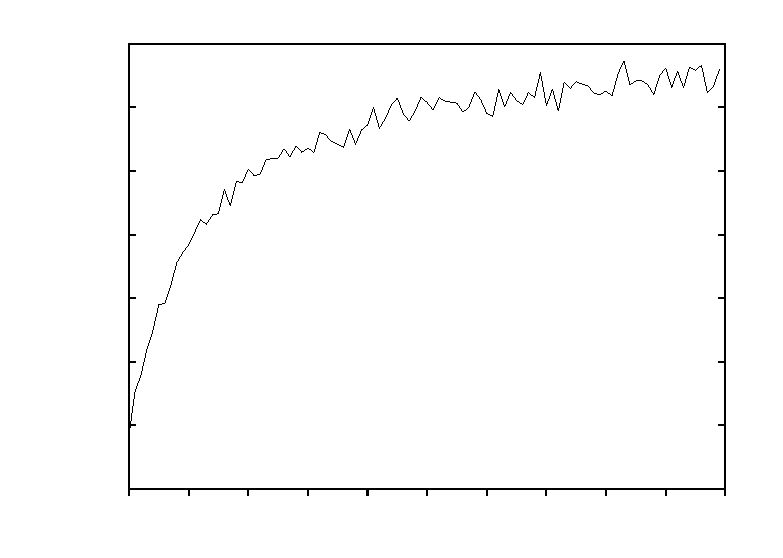
\includegraphics{tauoptoverpred}}%
    \gplfronttext
  \end{picture}%
\endgroup
}
\bigskip
\rule{33em}{0.5pt}
\caption{\label{predovertauopt} This figure shows the ratio of the predicted value for $\tau$ in an exponential model over the empirical optimised value $\tau_o$.}
\end{center}
\end{figure}

This leads to the following ordinary differential equation:

\begin{equation}
\frac{dy}{dt}(t) = \left( r - d - u - \lambda_u \right)y(t) + u
\end{equation}

This ODE has general solution:
\begin{equation}
y(t) = Ce^{(r-d-u-\lambda_u)(t-t_0)} + \frac{u}{u+d+\lambda_u - r}
\end{equation}

Since $y(t_0) = 1$, get:
\begin{equation}
y(t) = \frac{d+\lambda_u - r}{d+u+\lambda_u -r} e^{(r-d-u-\lambda_u)(t-t_0)} + \frac{u}{u+d+\lambda_u-r}
\end{equation}

Letting $\lambda_u = r(u+d)/u$, get:
\begin{equation}
y(t) = \frac{d(u+r)}{u^2 + d(u+r)} e^{-\frac{u^2+d(u+r)}{u}(t-t_0)} + \frac{u^2}{u^2+ d(u+r)}
\end{equation}

This solution was tested against a standard exponential model, which was minimised over $\tau$ with a downhill simplex method \citep{NelderMead1965a}.  Downhill simplex is a non-parametric minimisation algorithm that searches the solution space through reflection and stretching of a simplex.

Figure \ref{predovertauopt} shows how the ratio of the predicted value for $\tau$ over the optimised value rises towards one as the value for $u$ increases.  This suggests that, while this method is clearly not completely correct, that it is at least a reasonable approximation.

\section{Markov Process}

The transition between the up and down states is defined only by the switching rates, and not the rate history. In this way, the rate process is a continuous-time Markov chain (CTMC).  That is, the future of the process does not depend on the past at all, merely whether the model is currently in the up-state or the down-state.

By the theory of Markov Chains, this process can be described by the simultaneous differential equations:
\begin{equation}
\left\{
\begin{split} &p_u^{\prime}(t) = -dp_u(t) + dp_d(t)\\ &p_d^{\prime}(t)=up_u(t) - up_d(t)
\end{split}
\right.
\end{equation}
This is simply the linear ODE:
\begin{equation}
P^{\prime}(t) = P(t)Q
\end{equation}
where
\begin{equation}
Q =  \begin{pmatrix} -d & d \\ u & -u \end{pmatrix}
\end{equation}

Then the solution to the matrix $P(t)$ is simply the exponential of the transition matrix, $Q$:
\begin{equation}
P(t) = e^{tQ}.
\end{equation}

The solution to the Markov chain of rates is then:
\begin{equation}
P(t) = e^{tQ} = \begin{pmatrix} \frac{u}{u+d}+\frac{d}{u+d}e^{-(u+d)t} & \frac{d}{u+d} - \frac{d}{u+d}e^{-(u+d)t} \\ \frac{u}{u+d} - \frac{u}{u+d}e^{-(u+d)t} & \frac{d}{u+d} + \frac{u}{u+d}e^{-(u+d)t}\end{pmatrix}
\end{equation}

In order to calculate the probability of being in the up-state at a time $t$ after a spike at $t=0$, it is necessary to introduce another state to the Markov chain.  At any time $t$ between two spikes, $t=0$ and $t=t_1$ say, there is implicit knowledge that there was a spike at time $t=0$, and that there has not been a spike since.  If the spiking state is treated as the end of the particular Markov chain, as a default is in financial mathematics \citep{KijimaKomoribayashi1998a}, then, provided there has been no spike since $t=0$, it suffices to calculate the exponential of the transition matrix $Q_s$ below:

\begin{equation}
Q_s = \begin{pmatrix} -d-\lambda_u & d & \lambda_u \\ u & -u & 0 \\ 0 & 0 & 0\end{pmatrix}
\end{equation}

The third state of the Markov chain described by the transition matrix $Q_s$ is an ``absorbing'' state, the state of spiking, from which it is impossible to return to either the up or the down state.

\begin{figure}[htb]
\begin{center}
\setlength{\unitlength}{.07cm}
\begin{picture}(120,75)
\put(90,37){\mbox{$\lambda_d$}}
\put(25,37){\mbox{$\lambda_u$}}
\put(59,67){\mbox{$d$}}
\put(59,49){\mbox{$u$}}

\put(25,60){\oval(40,25)}
\put(21,58){\mbox{{\bf UP}}}
\put(95,60){\oval(40,25)}
\put(85,58){\mbox{{\bf DOWN}}}
\put(60,20){\oval(40,25)}
\put(51,18){\mbox{{\bf SPIKE}}}

\put(45,65){\vector(1,0){30}}
\put(75,55){\vector(-1,0){30}}
\put(25,47.5){\vector(4,-3){21}}
\put(95,47.5){\vector(-4,-3){21}}
\end{picture}
\bigskip
\rule{33em}{0.5pt}
\caption{\label{markov} An illustration of the state space of the Markov chain at any point in time between two spikes.}
\end{center}
\end{figure}


The solution to the spiking Markov chain is:
\begin{equation}
P(t)  = \begin{pmatrix} Ae^{-\alpha t} + (1-A)e^{-\beta t} & Be^{-\alpha t} - Be^{-\beta t} & p_{13}(t)\\ 
Ce^{-\alpha t} - Ce^{-\beta t} & (1-A)e^{-\alpha t} +  Ae^{-\beta t} & p_{23}(t) \\
 0 & 0 & 1 \end{pmatrix}
\end{equation}
where $-\alpha,-\beta$ are the roots to the characteristic polynomial of $Q_s$, and $p_{13}(t), p_{23}(t)$ are such that their rows sum to one.
\begin{equation}
\begin{split}
-\alpha = \frac{-(u+d+\lambda_u) + \sqrt{(u-d-\lambda_u)^2 + 4ud}}{2}\\
-\beta = \frac{-(u+d+\lambda_u) - \sqrt{(u-d-\lambda_u)^2 + 4ud}}{2}
\end{split}
\end{equation}
Since $u,d,\lambda_u >0$, these probabilities are simply double exponentials, and there are no trigonometric terms.

Specifically:
\begin{equation}
\begin{split}
&A = \frac{\left(u-d-\lambda_u+\sqrt{(u-d-\lambda_u)^2+4ud}\right)}{2\sqrt{(u-d-\lambda_u)^2+4ud}}\\
&B = \frac{d}{\sqrt{(u-d-\lambda_u)^2+4ud}}\\
&C = \frac{u}{\sqrt{(u-d-\lambda_u)^2+4ud}}
\end{split}
\end{equation}
It can be  easily confirmed that $A,B,C>0$, which is necessary to ensure that all the probabilities are between 0 and 1.

If the model is changed such that there is a non-zero spiking probability, $\lambda_d>0$, in the down-state, then the transition matrix $Q_s$ becomes:
\begin{equation}
Q_s = \begin{pmatrix} -d-\lambda_u & d & \lambda_u \\ u & -u-\lambda_d & \lambda_d \\ 0 & 0 & 0 \end{pmatrix}
\end{equation}

This matrix has solution:
\begin{equation}
P_s(t) =
\begin{pmatrix}
Ae^{-\alpha t} + (1-A)e^{-\beta t} & B\left(e^{-\alpha t} - e^{-\beta t}\right) & p_{13}(t) \\
C\left(e^{-\alpha t} - e^{-\beta t}\right) & (1-A)e^{-\alpha t} + Ae^{-\beta t} & p_{23}(t)\\
0 & 0 & 1
\end{pmatrix}
\end{equation}
where $-\alpha,-\beta$ are once again the roots of the characteristic polynomial of $Q_s$.
\begin{equation}
\begin{split}
-\alpha = \frac{-(u+d+\lambda_u+\lambda_d) + \sqrt{(u-d+\lambda_d-\lambda_u)^2+4ud}}{2}\\
-\beta = \frac{-(u+d+\lambda_u+\lambda_d) - \sqrt{(u-d+\lambda_d-\lambda_u)^2+4ud}}{2}
\end{split}
\end{equation}
again, $u,d>0$ means that the probabilities above are all double exponentials, with no trigonometric terms.

\begin{equation}
\begin{split}
& A = \frac{u-d+\lambda_d-\lambda_u + \sqrt{(u-d+\lambda_d-\lambda_u)^2+4ud}}{2\sqrt{(u-d+\lambda_d-\lambda_u)^2 + 4ud}}\\
& B = \frac{d}{\sqrt{(u-d+\lambda_d-\lambda_u)^2 + 4ud}}\\
& C = \frac{u}{\sqrt{(u-d+\lambda_d-\lambda_u)^2 + 4ud}}
\end{split}
\end{equation}

To simplify notation, set:
\begin{equation}
\begin{split}
\label{dg}
\Delta &= \lambda_u - \lambda_d\\
\gamma &= \sqrt{(u-d-\Delta)^2 + 4ud}
\end{split}
\end{equation}

Thus:
\begin{equation}
\begin{split}
A = \frac{u-d - \Delta + \gamma}{2\gamma},\, B = \frac{d}{\gamma}, \,C = \frac{u}{\gamma}
\end{split}
\end{equation}

\subsection{Estimating the rate function $r(t)$}

These probabilities can now be used to calculate the estimated rate function, $r(t)$, based on the timing of spikes.  Assuming that the probability of the last spike is known, then the rate function between any two spikes is estimated by this Markov model. 

If the probability vector at the time of the last spike is ${\bf p_0}=(p_0, 1-p_0,0)$, then the probabilities at a time $t$ after the spike are:
\begin{equation}
{\bf p(t)} = {\bf p_0}e^{Q_s} = (p_u(t),p_d(t),p_s(t))
\end{equation}
where
\begin{equation}
\begin{split}
p_u(t) &= (p_0(A-C)+C)e^{-\alpha t}+(p_0(1-A+C)-C)e^{-\beta t}\\
p_d(t) &= (p_0(A+B-1)+1-A)e^{-\alpha t}+(p_0(-A-B)+A)e^{-\beta t}\\
p_s(t) &= 1 - p_u(t) - p_d(t)
\end{split}
\end{equation}

The probabilities $p_u(t), \,p_d(t)$ represent the probability of being in the up/down state and not spiking.  The probability required to calculate the rate function, $r(t)$, between spikes is the probability of being in the up-state given that there has not been a spike.  This is because it is known that there has been no spike since the last spike.  Therefore, by Baye's Theorem, the probability $p(t)$ is just:
\begin{equation}
p(t)  = \frac{p_u(t)}{p_u(t) + p_d(t)}
\end{equation}
so, the rate function becomes:
\begin{equation}\label{roft}
r(t) = \Delta p(t) + \lambda_d = \frac{A_0e^{-\alpha t}+B_0e^{-\beta t}}{C_0e^{-\alpha t} + D_0e^{\beta t}}
\end{equation}
where:
\begin{equation}
\begin{split}
\label{abcd}
A_0 & = \Delta(p_0(-u-d-\Delta + \gamma)+2u)+\lambda_dC_0\\
B_0 & =\Delta(p_0(u+d+\Delta + \gamma)-2u)+\lambda_dD_0\\
C_0 & = p_0(-2\Delta)+u+d+\Delta+\gamma\\
D_0 & = p_0(2\Delta) -u-d-\Delta + \gamma
\end{split}
\end{equation}

Since $-\beta<-\alpha$, this can be written as:
\begin{equation}
r(t) = \frac{A_0+B_0e^{-\gamma t}}{C_0 + D_0e^{-\gamma t}}
\end{equation}
so the asymptotic value of $r(t)$ is equal to the fraction $A_0/C_0$, so this value should not depend on $p_0$.  Allowing $\delta=u+d+\Delta$, then $\delta^2 -4u\Delta= \gamma^2$ which simplifies the calculation.

$A_0 = 2\Delta u + p_0\Delta(\gamma-\delta) + \lambda_d C_0$, and $C_0 = \gamma + \delta -2\Delta p_0$:

\begin{equation}
\Delta p_0 = -\frac{C_0 - \gamma - \delta}{2}
\end{equation}
then
\begin{equation}
A_0 = 2\Delta u - \frac{1}{2}C_0(\gamma-\delta - 2\lambda_d) +\frac{1}{2}(\gamma+\delta)(\gamma-\delta)
\end{equation}

Therefore:
\begin{equation}
\frac{A_0}{C_0} = \lambda_d + \frac{1}{2}(\delta-\gamma) = \alpha
\end{equation}

similarly
\begin{equation}
\frac{B_0}{D_0} = \lambda_d + \frac{1}{2}(\gamma+\delta) = \beta
\end{equation}

This can be viewed as the asymptotic value of the rate as time goes to $-\infty$.

So the rate function $r(t)$ simplifies to:
\begin{equation}\label{rate}
r(t) = \frac{\alpha C_0 + \beta D_0e^{-\gamma t}}{C_o + D_0e^{-\gamma t}} = \frac{\alpha C_0e^{-\alpha t} + \beta D_0e^{-\beta t}}{C_oe^{-\alpha t} + D_0e^{-\beta t}} 
\end{equation}

In fact, comparing $C_0$ to $\beta$ and $D_0$ to $\alpha$, get:
\begin{equation}
\begin{split}
C_0 = 2(\beta - \lambda_d - p_0\Delta), \\ 
D_0 = 2(-\alpha + \lambda_d + p_0\Delta)
\end{split}
\end{equation}

Remembering that $p_0$ is just the probability of being in the up-state at $t=0$, then:
\begin{equation}
\Delta p_0 + \lambda_d = r(0),
\end{equation}
that is, the firing rate at $t=0$.  Then the equation \ref{rate}, the firing rate at time $t$, simplifies to:
\begin{equation}
r(t) = \frac{\alpha(\beta - r(0))e^{-\alpha t} + \beta(r(0)-\alpha)e^{-\beta t}}{(\beta - r(0))e^{-\alpha t} + (r(0)-\alpha)e^{-\beta t}}
\end{equation}

\subsection{Change in probability when a spike arrives}

In the previous section, the rate function, $r(t)$, and the probability density function of the ISI distribution, $p_{ISI}(t)$, were calculated, given that the probability of being in the up-state at the time of the last spike, $p_0$, is known.  However, it is necessary to re-evaluate the probability at the time a spike arrives.

If the probability of being in the up-state before the spike is $p_u(t)$, then the presence of a spike provides information on the state of the model. By Baye's Theorem:

\begin{equation}
\begin{split}
P(\mbox{up-state} | \mbox{spike}) &= \frac{P(\mbox{spike}|\mbox{up-state})P(\mbox{up-state})}{P(\mbox{spike})} \\
&=\frac{\lambda_u p_u(t)}{\Delta p_u(t) + \lambda_d }
\end{split}
\end{equation}

Thus:
\begin{equation}
p_u(t) \rightarrow \frac{\lambda_u p_u(t)}{\Delta p(t) + \lambda_d}
\end{equation}

equivalently:
\begin{equation}
\begin{split}
r(t) \rightarrow &(\lambda_u - \lambda_d)\frac{\lambda_u p_u(t)}{\Delta p_u(t)+ \lambda_d} + \lambda_d\\
= & \frac{\lambda_u^2 p_u(t) + \lambda_d^2(1-p_u(t))}{\lambda_up_u(t) + \lambda_d(1-p_u(t))}
\end{split}
\end{equation}

Equivalently, this can be written as:
\begin{equation}
r(t) \rightarrow (\lambda_u +\lambda_d) - \frac{\lambda_u\lambda_d}{r(t)}
\end{equation}

\begin{figure}[htb]
% GNUPLOT: LaTeX picture with Postscript
\begingroup
  \makeatletter
  \providecommand\color[2][]{%
    \GenericError{(gnuplot) \space\space\space\@spaces}{%
      Package color not loaded in conjunction with
      terminal option `colourtext'%
    }{See the gnuplot documentation for explanation.%
    }{Either use 'blacktext' in gnuplot or load the package
      color.sty in LaTeX.}%
    \renewcommand\color[2][]{}%
  }%
  \providecommand\includegraphics[2][]{%
    \GenericError{(gnuplot) \space\space\space\@spaces}{%
      Package graphicx or graphics not loaded%
    }{See the gnuplot documentation for explanation.%
    }{The gnuplot epslatex terminal needs graphicx.sty or graphics.sty.}%
    \renewcommand\includegraphics[2][]{}%
  }%
  \providecommand\rotatebox[2]{#2}%
  \@ifundefined{ifGPcolor}{%
    \newif\ifGPcolor
    \GPcolorfalse
  }{}%
  \@ifundefined{ifGPblacktext}{%
    \newif\ifGPblacktext
    \GPblacktexttrue
  }{}%
  % define a \g@addto@macro without @ in the name:
  \let\gplgaddtomacro\g@addto@macro
  % define empty templates for all commands taking text:
  \gdef\gplbacktext{}%
  \gdef\gplfronttext{}%
  \makeatother
  \ifGPblacktext
    % no textcolor at all
    \def\colorrgb#1{}%
    \def\colorgray#1{}%
  \else
    % gray or color?
    \ifGPcolor
      \def\colorrgb#1{\color[rgb]{#1}}%
      \def\colorgray#1{\color[gray]{#1}}%
      \expandafter\def\csname LTw\endcsname{\color{white}}%
      \expandafter\def\csname LTb\endcsname{\color{black}}%
      \expandafter\def\csname LTa\endcsname{\color{black}}%
      \expandafter\def\csname LT0\endcsname{\color[rgb]{1,0,0}}%
      \expandafter\def\csname LT1\endcsname{\color[rgb]{0,1,0}}%
      \expandafter\def\csname LT2\endcsname{\color[rgb]{0,0,1}}%
      \expandafter\def\csname LT3\endcsname{\color[rgb]{1,0,1}}%
      \expandafter\def\csname LT4\endcsname{\color[rgb]{0,1,1}}%
      \expandafter\def\csname LT5\endcsname{\color[rgb]{1,1,0}}%
      \expandafter\def\csname LT6\endcsname{\color[rgb]{0,0,0}}%
      \expandafter\def\csname LT7\endcsname{\color[rgb]{1,0.3,0}}%
      \expandafter\def\csname LT8\endcsname{\color[rgb]{0.5,0.5,0.5}}%
    \else
      % gray
      \def\colorrgb#1{\color{black}}%
      \def\colorgray#1{\color[gray]{#1}}%
      \expandafter\def\csname LTw\endcsname{\color{white}}%
      \expandafter\def\csname LTb\endcsname{\color{black}}%
      \expandafter\def\csname LTa\endcsname{\color{black}}%
      \expandafter\def\csname LT0\endcsname{\color{black}}%
      \expandafter\def\csname LT1\endcsname{\color{black}}%
      \expandafter\def\csname LT2\endcsname{\color{black}}%
      \expandafter\def\csname LT3\endcsname{\color{black}}%
      \expandafter\def\csname LT4\endcsname{\color{black}}%
      \expandafter\def\csname LT5\endcsname{\color{black}}%
      \expandafter\def\csname LT6\endcsname{\color{black}}%
      \expandafter\def\csname LT7\endcsname{\color{black}}%
      \expandafter\def\csname LT8\endcsname{\color{black}}%
    \fi
  \fi
  \setlength{\unitlength}{0.0500bp}%
  \begin{picture}(7200.00,5040.00)%
    \gplgaddtomacro\gplbacktext{%
      \csname LTb\endcsname%
      \put(814,767){\makebox(0,0)[r]{\strut{} 0}}%
      \put(814,1496){\makebox(0,0)[r]{\strut{} 10}}%
      \put(814,2224){\makebox(0,0)[r]{\strut{} 20}}%
      \put(814,2953){\makebox(0,0)[r]{\strut{} 30}}%
      \put(814,3682){\makebox(0,0)[r]{\strut{} 40}}%
      \put(814,4411){\makebox(0,0)[r]{\strut{} 50}}%
      \put(946,484){\makebox(0,0){\strut{} 0}}%
      \put(2117,484){\makebox(0,0){\strut{} 0.2}}%
      \put(3289,484){\makebox(0,0){\strut{} 0.4}}%
      \put(4460,484){\makebox(0,0){\strut{} 0.6}}%
      \put(5632,484){\makebox(0,0){\strut{} 0.8}}%
      \put(6803,484){\makebox(0,0){\strut{} 1}}%
      \put(176,2771){\rotatebox{-270}{\makebox(0,0){\strut{}Rate (s^{-1})}}}%
      \put(3874,154){\makebox(0,0){\strut{}$t$ (s)}}%
    }%
    \gplgaddtomacro\gplfronttext{%
    }%
    \gplbacktext
    \put(0,0){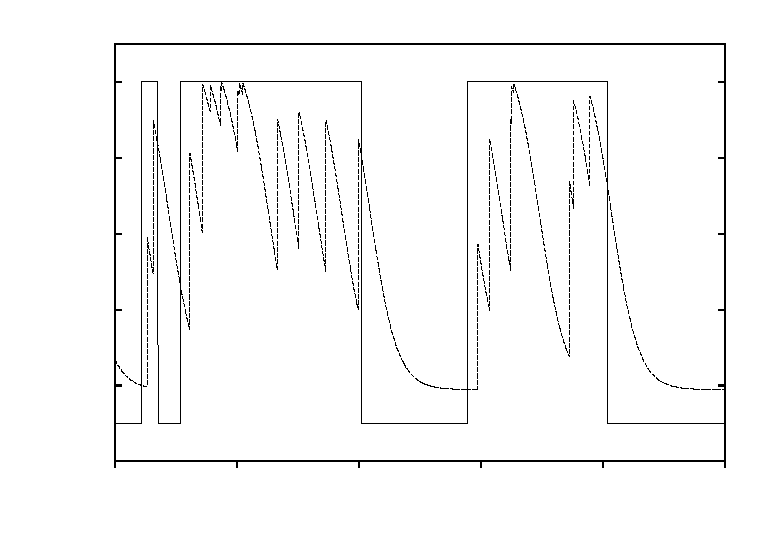
\includegraphics{estrate}}%
    \gplfronttext
  \end{picture}%
\endgroup

\bigskip
\rule{33em}{0.5pt}
\caption{An example of the estimated rate, $r(t)$, for a bimodal Poisson spike train.  For this example, $u=d=5$, $\lambda_u=50$ and $\lambda_d=5$.  In this example, the initial rate was set randomly between $\alpha$ and $\beta$.}
\end{figure}

\begin{figure}
% GNUPLOT: LaTeX picture with Postscript
\begingroup
  \makeatletter
  \providecommand\color[2][]{%
    \GenericError{(gnuplot) \space\space\space\@spaces}{%
      Package color not loaded in conjunction with
      terminal option `colourtext'%
    }{See the gnuplot documentation for explanation.%
    }{Either use 'blacktext' in gnuplot or load the package
      color.sty in LaTeX.}%
    \renewcommand\color[2][]{}%
  }%
  \providecommand\includegraphics[2][]{%
    \GenericError{(gnuplot) \space\space\space\@spaces}{%
      Package graphicx or graphics not loaded%
    }{See the gnuplot documentation for explanation.%
    }{The gnuplot epslatex terminal needs graphicx.sty or graphics.sty.}%
    \renewcommand\includegraphics[2][]{}%
  }%
  \providecommand\rotatebox[2]{#2}%
  \@ifundefined{ifGPcolor}{%
    \newif\ifGPcolor
    \GPcolorfalse
  }{}%
  \@ifundefined{ifGPblacktext}{%
    \newif\ifGPblacktext
    \GPblacktexttrue
  }{}%
  % define a \g@addto@macro without @ in the name:
  \let\gplgaddtomacro\g@addto@macro
  % define empty templates for all commands taking text:
  \gdef\gplbacktext{}%
  \gdef\gplfronttext{}%
  \makeatother
  \ifGPblacktext
    % no textcolor at all
    \def\colorrgb#1{}%
    \def\colorgray#1{}%
  \else
    % gray or color?
    \ifGPcolor
      \def\colorrgb#1{\color[rgb]{#1}}%
      \def\colorgray#1{\color[gray]{#1}}%
      \expandafter\def\csname LTw\endcsname{\color{white}}%
      \expandafter\def\csname LTb\endcsname{\color{black}}%
      \expandafter\def\csname LTa\endcsname{\color{black}}%
      \expandafter\def\csname LT0\endcsname{\color[rgb]{1,0,0}}%
      \expandafter\def\csname LT1\endcsname{\color[rgb]{0,1,0}}%
      \expandafter\def\csname LT2\endcsname{\color[rgb]{0,0,1}}%
      \expandafter\def\csname LT3\endcsname{\color[rgb]{1,0,1}}%
      \expandafter\def\csname LT4\endcsname{\color[rgb]{0,1,1}}%
      \expandafter\def\csname LT5\endcsname{\color[rgb]{1,1,0}}%
      \expandafter\def\csname LT6\endcsname{\color[rgb]{0,0,0}}%
      \expandafter\def\csname LT7\endcsname{\color[rgb]{1,0.3,0}}%
      \expandafter\def\csname LT8\endcsname{\color[rgb]{0.5,0.5,0.5}}%
    \else
      % gray
      \def\colorrgb#1{\color{black}}%
      \def\colorgray#1{\color[gray]{#1}}%
      \expandafter\def\csname LTw\endcsname{\color{white}}%
      \expandafter\def\csname LTb\endcsname{\color{black}}%
      \expandafter\def\csname LTa\endcsname{\color{black}}%
      \expandafter\def\csname LT0\endcsname{\color{black}}%
      \expandafter\def\csname LT1\endcsname{\color{black}}%
      \expandafter\def\csname LT2\endcsname{\color{black}}%
      \expandafter\def\csname LT3\endcsname{\color{black}}%
      \expandafter\def\csname LT4\endcsname{\color{black}}%
      \expandafter\def\csname LT5\endcsname{\color{black}}%
      \expandafter\def\csname LT6\endcsname{\color{black}}%
      \expandafter\def\csname LT7\endcsname{\color{black}}%
      \expandafter\def\csname LT8\endcsname{\color{black}}%
    \fi
  \fi
  \setlength{\unitlength}{0.0500bp}%
  \begin{picture}(7200.00,5040.00)%
    \gplgaddtomacro\gplbacktext{%
      \csname LTb\endcsname%
      \put(814,767){\makebox(0,0)[r]{\strut{} 0}}%
      \put(814,1496){\makebox(0,0)[r]{\strut{} 10}}%
      \put(814,2224){\makebox(0,0)[r]{\strut{} 20}}%
      \put(814,2953){\makebox(0,0)[r]{\strut{} 30}}%
      \put(814,3682){\makebox(0,0)[r]{\strut{} 40}}%
      \put(814,4411){\makebox(0,0)[r]{\strut{} 50}}%
      \put(946,484){\makebox(0,0){\strut{} 0}}%
      \put(2117,484){\makebox(0,0){\strut{} 0.2}}%
      \put(3289,484){\makebox(0,0){\strut{} 0.4}}%
      \put(4460,484){\makebox(0,0){\strut{} 0.6}}%
      \put(5632,484){\makebox(0,0){\strut{} 0.8}}%
      \put(6803,484){\makebox(0,0){\strut{} 1}}%
      \put(176,2771){\rotatebox{-270}{\makebox(0,0){\strut{}Rate (s^{-1})}}}%
      \put(3874,154){\makebox(0,0){\strut{}$t$ (s)}}%
    }%
    \gplgaddtomacro\gplfronttext{%
    }%
    \gplbacktext
    \put(0,0){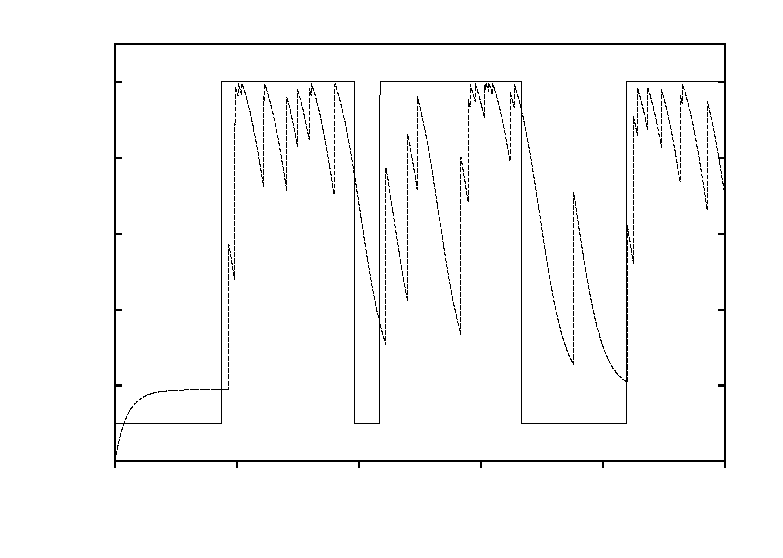
\includegraphics{estrate2}}%
    \gplfronttext
  \end{picture}%
\endgroup

\bigskip
\rule{33em}{0.5pt}
\caption{An example of the estimated rate, $r(t)$, for a bimodal Poisson spike train.  For this example, $u=d=5$, $\lambda_u=50$ and $\lambda_d=5$.  In this example, the initial rate was set to zero and it subsequently set itself.}
\end{figure}

\subsection{Calculating the ISI distribution}

When dealing with spike-train data, it is very useful to know the inter-spike interval (ISI) distribution, as this can be observed much easier than the firing rate of a neuron.

The probability density function of the ISI distribution of an inhomogeneous Poisson process, with rate function $r(t)$, is:
\begin{equation}
p_{ISI}(t) = r(t) e^{-\int_0^t r(s)\,ds}
\end{equation}

Now it is necessary to integrate the rate function from $0$ to $t$:
\begin{equation}
\begin{split}
\label{int}
&\int_0^t r(s)\,ds = \int_0^t  \frac{\alpha C_0e^{-\alpha s}+\beta D_0e^{-\beta s}}{C_0e^{-\alpha s} + D_0e^{\beta s}}\,ds\\ 
&= \frac{\alpha^2 C_0D_0 - \beta^2 C_0D_0}{(\alpha - \beta)C_0D_0}t + \frac{\beta C_0D_0-\alpha C_0D_0}{(\alpha - \beta)C_0D_0} \log\left({\frac{C_0e^{\beta t} + D_0e^{\alpha t}}{C_0 + D_0} }\right)
\end{split}
\end{equation}

Since $C_0$ and $D_0$ are not equal to zero, the fractions in the above equation become:
\begin{equation}
\begin{split}
\frac{\alpha^2 C_0D_0 - \beta^2 C_0D_0}{(\alpha - \beta)C_0D_0} & = \alpha+\beta,\\
 \frac{ \beta C_0D_0-\alpha A_0D_0}{(\alpha - \beta)C_0D_0} &= -1
\end{split}
\end{equation}
Thus equation \ref{int} becomes:
\begin{equation}
\begin{split}
\int_0^t r(s)\,ds &= (\alpha+\beta)t - \log\left( {\frac{C_0e^{\beta t} + D_0e^{\alpha t}}{C_0 + D_0} }\right) \\
&= \log \left( \frac{C_0+D_0}{C_0e^{-\alpha t}+D_0e^{-\beta t}}\right)
\end{split}
\end{equation}

Now $p_{ISI}(t)$ becomes:
\begin{equation}
\begin{split}
p_{ISI}(t) &= \frac{A_0e^{-\alpha t}+B_0e^{-\beta t}}{C_0e^{-\alpha t} + D_0e^{-\beta t}}e^{-\log \left( \frac{C_0+D_0}{C_0e^{-\alpha t}+D_0e^{-\beta t}}\right)}\\
&= \frac{A_0}{C_0+D_0}e^{-\alpha t} + \frac{B_0}{C_0+D_0}e^{-\beta t}
\end{split}
\end{equation}

This is the probability density function (pdf) of a hyper-exponential distribution, $H_2$, which has typical probability density function:
\begin{equation}
f(x) = \rho\lambda_1 e^{-\lambda_1 x} + (1-\rho) e^{-\lambda_2 x}
\end{equation}

Clearly, then $\lambda_1, \lambda_2$ which are calculated experimentally correspond to $\alpha,\beta$.  If $\lambda_1 = \alpha$ and $\lambda_2 = \beta$, then it is possible to derive the terms $C_0$ and $D_0$ from equation \ref{rate} for the probabilistic rate function:
\begin{equation}
C_0 = 2p(\lambda_2-\lambda_1), \, D_0 = 2(1-p)(\lambda_2-\lambda_1)
\end{equation}


\section{Testing on data}
The expectation of a hyperexponential ISI distribution allows for testing on real data.  The data used in this report is the data used in \citep{NarayanEtAl2006b}.  An electrode was placed in L1 of anaesthetised zebra finches, and the birds were presented with 20 natural stimuli ten times each.  As the model does not account for the refractory period of neurons, a well-documented feature of neurons \citep{OlshausenField2004a} , the ten presentations of each stimulus are overlaid to counter the impact of the refractory period \citep{BerryMeister1998a}. 

The inter-spike intervals (ISIs) were then aggregated across 16 of the 20 stimuli, to give a representation of a typical ISI distribution for each neuron.  The hyperexponential distribution, $H_2$, was trained on the ISI distribution of the 16 stimuli by minimising the statistic $D_n$ of the Kolmogorov-Smirnov test \citep{Massey1951a} by downhill-simplex search.  Then the remaining four stimuli were aggregated across the ten trials to form a test ISI distribution upon which the calculated minimum hyperexponential distribution was tested using the Kolmogorov-Smirnov test for goodness-of-fit.

\begin{figure}
% GNUPLOT: LaTeX picture with Postscript
\begingroup
  \makeatletter
  \providecommand\color[2][]{%
    \GenericError{(gnuplot) \space\space\space\@spaces}{%
      Package color not loaded in conjunction with
      terminal option `colourtext'%
    }{See the gnuplot documentation for explanation.%
    }{Either use 'blacktext' in gnuplot or load the package
      color.sty in LaTeX.}%
    \renewcommand\color[2][]{}%
  }%
  \providecommand\includegraphics[2][]{%
    \GenericError{(gnuplot) \space\space\space\@spaces}{%
      Package graphicx or graphics not loaded%
    }{See the gnuplot documentation for explanation.%
    }{The gnuplot epslatex terminal needs graphicx.sty or graphics.sty.}%
    \renewcommand\includegraphics[2][]{}%
  }%
  \providecommand\rotatebox[2]{#2}%
  \@ifundefined{ifGPcolor}{%
    \newif\ifGPcolor
    \GPcolorfalse
  }{}%
  \@ifundefined{ifGPblacktext}{%
    \newif\ifGPblacktext
    \GPblacktexttrue
  }{}%
  % define a \g@addto@macro without @ in the name:
  \let\gplgaddtomacro\g@addto@macro
  % define empty templates for all commands taking text:
  \gdef\gplbacktext{}%
  \gdef\gplfronttext{}%
  \makeatother
  \ifGPblacktext
    % no textcolor at all
    \def\colorrgb#1{}%
    \def\colorgray#1{}%
  \else
    % gray or color?
    \ifGPcolor
      \def\colorrgb#1{\color[rgb]{#1}}%
      \def\colorgray#1{\color[gray]{#1}}%
      \expandafter\def\csname LTw\endcsname{\color{white}}%
      \expandafter\def\csname LTb\endcsname{\color{black}}%
      \expandafter\def\csname LTa\endcsname{\color{black}}%
      \expandafter\def\csname LT0\endcsname{\color[rgb]{1,0,0}}%
      \expandafter\def\csname LT1\endcsname{\color[rgb]{0,1,0}}%
      \expandafter\def\csname LT2\endcsname{\color[rgb]{0,0,1}}%
      \expandafter\def\csname LT3\endcsname{\color[rgb]{1,0,1}}%
      \expandafter\def\csname LT4\endcsname{\color[rgb]{0,1,1}}%
      \expandafter\def\csname LT5\endcsname{\color[rgb]{1,1,0}}%
      \expandafter\def\csname LT6\endcsname{\color[rgb]{0,0,0}}%
      \expandafter\def\csname LT7\endcsname{\color[rgb]{1,0.3,0}}%
      \expandafter\def\csname LT8\endcsname{\color[rgb]{0.5,0.5,0.5}}%
    \else
      % gray
      \def\colorrgb#1{\color{black}}%
      \def\colorgray#1{\color[gray]{#1}}%
      \expandafter\def\csname LTw\endcsname{\color{white}}%
      \expandafter\def\csname LTb\endcsname{\color{black}}%
      \expandafter\def\csname LTa\endcsname{\color{black}}%
      \expandafter\def\csname LT0\endcsname{\color{black}}%
      \expandafter\def\csname LT1\endcsname{\color{black}}%
      \expandafter\def\csname LT2\endcsname{\color{black}}%
      \expandafter\def\csname LT3\endcsname{\color{black}}%
      \expandafter\def\csname LT4\endcsname{\color{black}}%
      \expandafter\def\csname LT5\endcsname{\color{black}}%
      \expandafter\def\csname LT6\endcsname{\color{black}}%
      \expandafter\def\csname LT7\endcsname{\color{black}}%
      \expandafter\def\csname LT8\endcsname{\color{black}}%
    \fi
  \fi
  \setlength{\unitlength}{0.0500bp}%
  \begin{picture}(7200.00,5040.00)%
    \gplgaddtomacro\gplbacktext{%
      \csname LTb\endcsname%
      \put(1078,767){\makebox(0,0)[r]{\strut{} 0}}%
      %\put(1078,1219){\makebox(0,0)[r]{\strut{} 0.02}}%
      \put(1078,1670){\makebox(0,0)[r]{\strut{} 0.04}}%
      %\put(1078,2122){\makebox(0,0)[r]{\strut{} 0.06}}%
      \put(1078,2573){\makebox(0,0)[r]{\strut{} 0.08}}%
      %\put(1078,3025){\makebox(0,0)[r]{\strut{} 0.1}}%
      \put(1078,3476){\makebox(0,0)[r]{\strut{} 0.12}}%
      %\put(1078,3928){\makebox(0,0)[r]{\strut{} 0.14}}%
      \put(1078,4379){\makebox(0,0)[r]{\strut{} 0.16}}%
      \put(2656,484){\makebox(0,0){\strut{} (a)}}%
      \put(4038,484){\makebox(0,0){\strut{} (b)}}%
      \put(5421,484){\makebox(0,0){\strut{} (c)}}%
      \put(176,2573){\makebox(0,0){\strut{}D_n}}%
      \put(4038,154){\makebox(0,0){\strut{}Distributions}}%
      \put(4038,4709){\makebox(0,0){\strut{}Kolmogorov-Smirnov statistics}}%
    }%
    \gplgaddtomacro\gplfronttext{%
    }%
    \gplbacktext
    \put(0,0){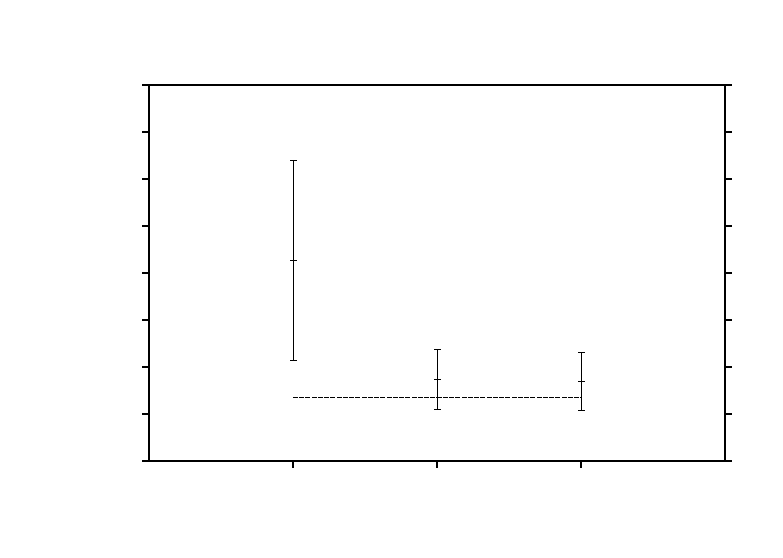
\includegraphics{ksdists}}%
    \gplfronttext
  \end{picture}%
\endgroup

\bigskip
\rule{33em}{0.5pt}
\caption{\label{exphehe3} The Kolmogorov-Smirnov test statistic $D_n$ for (a) the exponential distribution, (b) the hyperexponential distribution with two modes, and (c) the hyperexponential distribution with three modes.  The mean of the $p<0.05$ critical value is indicated by the broken line.}
\end{figure}

The Kolmogorov-Smirnov (KS) test is a nonparametric goodness-of-fit test introduced in \citep{Massey1951a}, based on results from \citet{Kolmogorov1933a} and \citet{Smirnoff1939a}.  It is used to compare a model probability distribution to a sample.  The KS statistic is the $d_{\infty}$ metric between the cumulative distribution function of the model distribution and the empirical distribution function of the data.
\begin{equation}
D_n = \sup_x \left| \hat{F}_n(x) - F(x) \right|
\end{equation}
where $\hat{F}_n(x)$ is the empirical distribution function of the data set of $n$ points and $F(x)$ is the cumulative distribution function of the proposed probability distribution.

Then the ISI distributions were tested against the hyperexponential distribution with both two and three modes $(H_2$ and $H_3)$.  As the exponential distribution is a special case of the hyperexponential distribution, and $H_2$ is a special case of $H_3$, it is clear that there should be an improvement with each step.  What was observed, as shown in Figure \ref{exphehe3}, was that the $H_2$ distribution was a drastic improvement on the exponential distribution, but the improvement of $H_3$ over $H_2$ was insignificant. 


At the $p<0.05$ significance level, only three out of $24$ neurons were not rejected by the Kolmogorov-Smirnov test for both the $H_2$ and the $H_3$ distributions. This could be due to the number of data points, which would make the KS test extremely rigorous.  It is also notable that this model is simply a first approximation to a neuron model; the KS statistic serves as a metric to determine goodness-of-fit rather than fitting the exact ISI distribution.

This seems to demonstrate that there is a bimodality of firing rates in neurons in the auditory forebrain of zebra finches.  This may suggest a sparse coding of features in the auditory forebrain of songbirds.  

